\documentclass[11pt,a4paper]{article}
\usepackage[T1]{fontenc}
\usepackage[utf8]{inputenc}
\usepackage{lmodern}
\usepackage[varqu,scaled=0.95]{zi4}
\usepackage[margin=2.3cm,headheight=14pt]{geometry}
\usepackage{microtype}
\usepackage{graphicx}
\usepackage{booktabs}
\usepackage{tabularx}
\usepackage{amsmath}
\usepackage{float}
\usepackage{placeins}
\usepackage{needspace}
\usepackage{xcolor}
\usepackage[parfill]{parskip}
\usepackage{enumitem}
\usepackage{titlesec}
\usepackage{fancyhdr}
\usepackage[font=small,labelfont={bf,color=accent},skip=6pt]{caption}
\usepackage{listings}
\usepackage[most]{tcolorbox}
\usepackage[colorlinks=true,linkcolor=accent,citecolor=accent,urlcolor=accent]{hyperref}

% ---------------------------------------------------------------------
% Colours (C/Java/Python match the figures)
\definecolor{accent}{HTML}{1F3A5F}
\definecolor{accentlight}{HTML}{EEF3F9}
\definecolor{rulegray}{HTML}{C9D3DF}
\definecolor{codebg}{HTML}{F8F9FB}
\definecolor{codekw}{HTML}{8A3FA0}
\definecolor{codecomment}{HTML}{6B7785}
\definecolor{langc}{HTML}{2A78D6}
\definecolor{langjava}{HTML}{EB6834}
\definecolor{langpython}{HTML}{1BAF7A}

% ---------------------------------------------------------------------
% Headings
\titleformat{\section}{\Needspace{8\baselineskip}\Large\bfseries\color{accent}}{\thesection}{0.7em}{}
  [\vspace{-4pt}{\color{rulegray}\titlerule[0.8pt]}]
\titlespacing*{\section}{0pt}{18pt}{10pt}
\titleformat{\subsection}{\Needspace{7\baselineskip}\large\bfseries\color{accent}}{\thesubsection}{0.6em}{}
\titlespacing*{\subsection}{0pt}{14pt}{6pt}

% A concept heading on its own line, with space above, inside a section
\newcommand{\concept}[1]{\par\addvspace{8pt}\Needspace{5\baselineskip}%
  \noindent{\color{accent}\bfseries\boldmath #1}\par\nopagebreak\vspace{2pt}}

% Page style
\pagestyle{fancy}
\fancyhf{}
\fancyhead[L]{\small\color{codecomment}Assignment 1 \textperiodcentered{} Matrix multiplication in C, Java and Python}
\fancyhead[R]{\small\color{codecomment}\AuthorName}
\fancyfoot[C]{\small\thepage}
\renewcommand{\headrulewidth}{0.4pt}
\renewcommand{\headrule}{{\color{rulegray}\hrule height\headrulewidth}}

% Lists
\setlist{itemsep=3pt,parsep=0pt,topsep=4pt}

% ---------------------------------------------------------------------
% Boxes
\newtcolorbox{infobox}[1][]{enhanced,breakable,colback=accentlight,colframe=accent,
  boxrule=0pt,leftrule=3pt,arc=0pt,left=10pt,right=10pt,top=6pt,bottom=6pt,
  before upper={\setlength{\parskip}{5pt}},#1}
\newtcolorbox{titledbox}[1]{enhanced,colback=accentlight,colframe=accent,
  boxrule=0.6pt,arc=2pt,left=10pt,right=10pt,top=6pt,bottom=6pt,
  title={\bfseries #1},fonttitle=\normalsize,coltitle=white,
  before upper={\setlength{\parskip}{5pt}}}

% Code listings
\lstdefinestyle{kernel}{
  basicstyle=\ttfamily\small,
  keywordstyle=\color{codekw}\bfseries,
  commentstyle=\color{codecomment}\itshape,
  stringstyle=\color{codecomment},
  numbers=left, numberstyle=\scriptsize\color{codecomment}, numbersep=8pt,
  showstringspaces=false, columns=fullflexible, keepspaces=true,
  aboveskip=0pt, belowskip=0pt, xleftmargin=14pt
}
\newtcblisting{codebox}[3]{enhanced,listing only,
  listing options={style=kernel,language=#1},
  colback=codebg,colframe=#3,boxrule=0.6pt,leftrule=3pt,arc=2pt,
  left=4pt,right=6pt,top=4pt,bottom=4pt,
  title={\ttfamily\small #2},coltitle=black,colbacktitle=#3!12,
  fonttitle=\bfseries,toptitle=1pt,bottomtitle=1pt}

% Tables
\renewcommand{\arraystretch}{1.12}

% ---------------------------------------------------------------------
% Generated by scripts/analyze.py -- do not edit by hand.
\newcommand{\TimeTable}{
\begin{tabular}{r l r r r r r}\toprule
$n$ & Language & Median & IQR (\%) & ns/iter & GFLOP/s & Batch \\\midrule
32 & C & 20.7 $\mu$s & 7.9 & 0.63 & 3.162 & 3509 \\
32 & Java & 28.6 $\mu$s & 1.8 & 0.87 & 2.295 & 334 \\
32 & Python & 2.71 ms & 19.9 & 82.58 & 0.024 & 29 \\
\addlinespace[2pt]
64 & C & 218.5 $\mu$s & 11.2 & 0.83 & 2.400 & 496 \\
64 & Java & 240.4 $\mu$s & 3.9 & 0.92 & 2.181 & 254 \\
64 & Python & 19.87 ms & 9.1 & 75.79 & 0.026 & 6 \\
\addlinespace[2pt]
128 & C & 3.37 ms & 1.4 & 1.61 & 1.244 & 30 \\
128 & Java & 1.75 ms & 6.1 & 0.83 & 2.400 & 51 \\
128 & Python & 154.92 ms & 4.8 & 73.87 & 0.027 & 1 \\
\addlinespace[2pt]
256 & C & 37.96 ms & 0.8 & 2.26 & 0.884 & 3 \\
256 & Java & 21.74 ms & 7.2 & 1.30 & 1.544 & 5 \\
256 & Python & 1.73 s & 17.4 & 103.18 & 0.019 & 1 \\
\addlinespace[2pt]
384 & C & 87.92 ms & 1.3 & 1.55 & 1.288 & 2 \\
384 & Java & 99.18 ms & 10.7 & 1.75 & 1.142 & 2 \\
384 & Python & 5.53 s & 2.9 & 97.60 & 0.020 & 1 \\
\addlinespace[2pt]
512 & C & 432.93 ms & 0.6 & 3.23 & 0.620 & 1 \\
512 & Java & 279.73 ms & 15.4 & 2.08 & 0.960 & 1 \\
512 & Python & 14.23 s & 9.2 & 106.03 & 0.019 & 1 \\
\addlinespace[2pt]
768 & C & 1.29 s & 3.3 & 2.85 & 0.703 & 1 \\
768 & Java & 1.22 s & 31.7 & 2.69 & 0.744 & 1 \\
768 & Python & 57.52 s & 8.9 & 126.99 & 0.016 & 1 \\
\addlinespace[2pt]
1024 & C & 5.48 s & 12.5 & 5.11 & 0.392 & 1 \\
1024 & Java & 4.27 s & 0.7 & 3.98 & 0.503 & 1 \\
1024 & Python & 95.07 s & 6.9 & 88.54 & 0.023 & 1 \\
\addlinespace[2pt]
1536 & C & 19.04 s & 0.5 & 5.25 & 0.381 & 1 \\
1536 & Java & 21.62 s & 0.3 & 5.97 & 0.335 & 1 \\
\addlinespace[2pt]
2048 & C & 48.46 s & 0.3 & 5.64 & 0.355 & 1 \\
2048 & Java & 45.19 s & 0.9 & 5.26 & 0.380 & 1 \\
\addlinespace[2pt]
\bottomrule\end{tabular}}
\newcommand{\MemoryTable}{
\begin{tabular}{r r r r r r r}\toprule
& \multicolumn{3}{c}{Peak working set (MB)} & \multicolumn{3}{c}{Storage model (MB)} \\\cmidrule(lr){2-4}\cmidrule(lr){5-7}
$n$ & C & Java & Python & C & Java & Python \\\midrule
32 & 4.1 & 58.4 & 19.1 & 0.0 & 0.0 & 0.1 \\
64 & 4.1 & 88.6 & 18.1 & 0.1 & 0.1 & 0.4 \\
128 & 4.6 & 79.5 & 20.2 & 0.4 & 0.4 & 1.6 \\
256 & 5.6 & 62.7 & 28.3 & 1.6 & 1.6 & 6.3 \\
384 & 7.5 & 68.7 & 46.2 & 3.5 & 3.6 & 14.2 \\
512 & 10.3 & 76.6 & 63.7 & 6.3 & 6.3 & 25.3 \\
768 & 18.2 & 116.2 & 113.7 & 14.2 & 14.2 & 56.8 \\
1024 & 29.2 & 152.1 & 187.2 & 25.2 & 25.2 & 100.8 \\
1536 & 60.6 & 262.5 & -- & 56.6 & 56.7 & -- \\
2048 & 104.7 & 373.8 & -- & 100.7 & 100.8 & -- \\
\bottomrule\end{tabular}}
\newcommand{\FitTable}{
\begin{tabular}{l r r}\toprule Language & Sizes used & Fitted exponent $b$ \\\midrule
C & 128--2048 (8 sizes) & 3.50 \\
Java & 128--2048 (8 sizes) & 3.73 \\
Python & 128--1024 (6 sizes) & 3.14 \\
\bottomrule\end{tabular}}
\newcommand{\ReplicationTable}{
\begin{tabular}{l r r r r}\toprule Language & $n$ & Main run & Replication & Change \\\midrule
C & 128 & 3.37 ms & 2.92 ms & -13\% \\
C & 256 & 37.96 ms & 36.49 ms & -4\% \\
C & 384 & 87.92 ms & 72.99 ms & -17\% \\
C & 512 & 432.93 ms & 683.97 ms & +58\% \\
C & 768 & 1.29 s & 1.17 s & -9\% \\
C & 1024 & 5.48 s & 5.46 s & -1\% \\
Java & 128 & 1.75 ms & 1.40 ms & -20\% \\
Java & 256 & 21.74 ms & 15.60 ms & -28\% \\
Java & 384 & 99.18 ms & 81.45 ms & -18\% \\
Java & 512 & 279.73 ms & 171.97 ms & -39\% \\
Java & 768 & 1.22 s & 649.18 ms & -47\% \\
Java & 1024 & 4.27 s & 3.76 s & -12\% \\
Python & 512 & 14.23 s & 9.31 s & -35\% \\
Python & 768 & 57.52 s & 42.12 s & -27\% \\
\bottomrule\end{tabular}}
\newcommand{\FlagsTable}{
\begin{tabular}{l r r r }\toprule GCC flags & $n=256$ & $n=512$ & $n=1024$ \\\midrule
O2 (main study) & 32.98 ms & 731.89 ms & 5.51 s \\
O2 {-}funroll{-}loops & 42.08 ms & 739.22 ms & 5.89 s \\
O3 & 36.23 ms & 700.88 ms & 5.50 s \\
O0 & 51.60 ms & 459.98 ms & 3.85 s \\
\bottomrule\end{tabular}}
\newcommand{\PaddingTable}{
\begin{tabular}{r r r r r}\toprule $n$ & C, pad 0 (row stride $8n$ B) & C, pad 2 ($8n+16$ B) & Speed-up & Java (main run) \\\midrule
128 & 3.06 ms & 1.34 ms & 2.3$\times$ & 1.75 ms \\
256 & 34.12 ms & 12.02 ms & 2.8$\times$ & 21.74 ms \\
384 & 77.16 ms & 41.47 ms & 1.9$\times$ & 99.18 ms \\
512 & 681.87 ms & 101.70 ms & 6.7$\times$ & 279.73 ms \\
768 & 1.17 s & 350.05 ms & 3.4$\times$ & 1.22 s \\
1024 & 5.96 s & 867.40 ms & 6.9$\times$ & 4.27 s \\
\bottomrule\end{tabular}}
\newcommand{\PaddingChecksumsEqual}{yes}


\newcommand{\AuthorName}{Amado Artiles Rodríguez}
\newcommand{\RepoURL}{https://github.com/amadoartiiles/matrix-multiplication-studies}

\hypersetup{pdftitle={Assignment 1: Basic Matrix Multiplication in C, Java and Python},
  pdfauthor={\AuthorName}}

\begin{document}

% =====================================================================
% Title block
\thispagestyle{empty}
\begin{tcolorbox}[enhanced,colback=accent,colframe=accent,coltext=white,arc=3pt,
  left=14pt,right=14pt,top=12pt,bottom=12pt]
{\small BIG DATA \quad\textperiodcentered\quad Grado en Ciencia e Ingeniería de Datos \quad\textperiodcentered\quad ULPGC \quad\textperiodcentered\quad 2026--2027}

\vspace{8pt}
{\LARGE\bfseries Assignment 1: Basic Matrix Multiplication\\[2pt] in C, Java and Python}

\vspace{8pt}
{\large How does matrix size affect the runtime and memory use of one triple-loop algorithm in three
languages?}
\end{tcolorbox}

\vspace{4pt}
\noindent{\large\bfseries \AuthorName}\hfill{\color{codecomment}October 2026}\\
{\small Repository: \url{\RepoURL}}

\vspace{6pt}
\begin{infobox}
{\color{accent}\bfseries Abstract}\par\vspace{3pt}
This study measures how the matrix size $n$ affects the runtime and peak memory of the same
$O(n^3)$ triple-loop multiplication of binary64 matrices in C, Java and Python, using identical
inputs, the same i-j-k loop order and the same timing boundary on one laptop (AMD Ryzen~7 7730U,
Windows~11), for $n=32$ to $2048$ with five measured repetitions each. All implementations gave
bitwise-identical results within a rigorous error bound of a NumPy reference. CPython was
17--130$\times$ slower than C, exceeded the 300\,s budget at $n=1536$ and grew close to $n^3$
(fitted exponent 3.14). C and Java stayed within a factor of two of each other but grew faster than
$n^3$ (3.50 and 3.73) as the matrices left the caches; padding each C row by 16 bytes made the same
code 1.9--6.9$\times$ faster, pointing to a memory-layout effect. Peak memory was dominated by the
runtime baseline for small $n$ and by the matrices for large $n$. The conclusions apply to these
implementations, settings and machine only.

\vspace{4pt}
{\small\textbf{Keywords:} matrix multiplication, benchmarking, C, Java, Python, cache effects,
memory layout.}
\end{infobox}

% =====================================================================
\section{Introduction and objective}

Dense matrix multiplication is the reference kernel of numerical computing and a common first
benchmark when comparing execution environments. Its textbook form performs exactly $n^3$
multiply-add operations for $n\times n$ inputs, so differences in runtime between implementations of
the \emph{same} algorithm expose the cost of the execution environment itself: interpretation, JIT
compilation, data representation and memory layout.

\begin{titledbox}{Research question}
\emph{For the straightforward triple-loop algorithm, how does the matrix size $n$ affect the runtime
and the peak memory of implementations in C, Java and Python on one fixed machine, and how does the
observed growth compare with the cubic model?}
\end{titledbox}

\concept{Hypotheses (stated before measuring)}
\begin{enumerate}[label=\textbf{H\arabic*}, leftmargin=2.2em]
  \item All three runtimes grow approximately as $n^3$ once fixed start-up costs are excluded.
  \item The compiled C version is fastest, Java is within a small factor of C after JIT warm-up, and
        CPython is one to two orders of magnitude slower because every inner iteration is
        interpreted.
  \item Memory grows as $n^2$; Python needs several times more memory per element than C and Java
        because each value is a separate heap object.
\end{enumerate}

% =====================================================================
\section{Background}

\concept{Algorithm}
$C_{ij}=\sum_{k=0}^{n-1}A_{ik}B_{kj}$ evaluated with three nested loops performs
$n^3$ multiplications and $n^3$ additions, i.e.\ $2n^3$ floating-point operations, and is
$\Theta(n^3)$ independent of the language \cite{golub}. In the i-j-k order the innermost loop reads a
row of $A$ with unit stride and a \emph{column} of $B$ with a stride of one row, which is the
cache-unfriendly access pattern that blocking and loop reordering later address \cite{lam,drepper}.

\concept{Floating point}
All three languages use IEEE~754 binary64 arithmetic \cite{ieee754}. Java has
had strict IEEE semantics for all floating-point operations since Java~17 \cite{jep306}; C compiled
without \texttt{-ffast-math} may not reassociate the sum; CPython's \texttt{float} is a C
\texttt{double}. Evaluating the same sums in the same order should therefore give identical results.

For a dot product of length $n$, the computed product satisfies, element-wise,
\[
  |\hat C - C|\le\gamma_n|A||B|, \qquad \gamma_n=\frac{nu}{1-nu}, \qquad u=2^{-53}
  \quad\text{\cite[Sec.~3.5]{higham}.}
\]

\concept{Execution environments}
C is compiled ahead of time to machine code. Java bytecode is first
interpreted and then compiled by the HotSpot JIT compiler, which is why warm-up runs are recommended
before measuring \cite{georges}. CPython interprets bytecode and represents each number as a boxed
heap object (24 bytes for a \texttt{float}, plus an 8-byte pointer in the list that holds it).

\concept{Caches}
The Zen~3 core of the test CPU has a 32\,KB 8-way L1 data cache and a 512\,KB 8-way
L2 cache per core, plus a 16\,MB L3 shared by eight cores \cite{amd}. When the distance between
consecutive accessed addresses is a large power of two, they map to only a few cache sets and evict
each other even though the cache is not full (conflict misses) \cite{lam,hennessy}.

% =====================================================================
\section{Methodology}

\subsection{Implementations}
The kernel is the same in the three languages (Figure~\ref{lst:kernels}). It allocates and
zero-initialises the result, then runs the i-j-k loop with a local accumulator \texttt{s}. No library
multiplication routine is called and no language-specific optimisation (loop hoisting, unrolling,
transposition) was written by hand.

\begin{figure}[H]
\begin{codebox}{C}{C \textperiodcentered{} c/matmul.c}{langc}
static double *multiply(const double *A, const double *B, int n) {
    double *C = (double *)calloc((size_t)n * n, sizeof(double));
    if (C == NULL) return NULL;
    for (int i = 0; i < n; i++) {
        for (int j = 0; j < n; j++) {
            double s = 0.0;
            for (int k = 0; k < n; k++) {
                s += A[(size_t)i * n + k] * B[(size_t)k * n + j];
            }
            C[(size_t)i * n + j] = s;
        }
    }
    return C;
}
\end{codebox}
\vspace{4pt}
\begin{codebox}{Java}{Java \textperiodcentered{} java/src/MatMul.java}{langjava}
static double[][] multiply(double[][] A, double[][] B, int n) {
    double[][] C = new double[n][n];
    for (int i = 0; i < n; i++) {
        for (int j = 0; j < n; j++) {
            double s = 0.0;
            for (int k = 0; k < n; k++) {
                s += A[i][k] * B[k][j];
            }
            C[i][j] = s;
        }
    }
    return C;
}
\end{codebox}
\vspace{4pt}
\begin{codebox}{Python}{Python \textperiodcentered{} python/matmul.py}{langpython}
def multiply(A, B, n):
    C = [[0.0] * n for _ in range(n)]
    for i in range(n):
        for j in range(n):
            s = 0.0
            for k in range(n):
                s += A[i][k] * B[k][j]
            C[i][j] = s
    return C
\end{codebox}
\caption{The timed kernels, exactly as in the repository (the timed region is the whole function).}
\label{lst:kernels}
\end{figure}

\concept{Storage layouts (unavoidable differences)}
\begin{itemize}[leftmargin=1.4em]
  \item \textbf{C:} one contiguous row-major \texttt{double} buffer per matrix ($8n^2$ bytes),
        allocated with \texttt{calloc}.
  \item \textbf{Java:} \texttt{double[n][n]}, an array of $n$ references to separately allocated row
        arrays; each row has a 16-byte object header, so consecutive rows are normally $8n+16$ bytes
        apart on the heap.
  \item \textbf{Python:} a list of $n$ row lists, each holding $n$ pointers to boxed \texttt{float}
        objects.
\end{itemize}
The analytical storage of $A$, $B$ and $C$ (``storage model'' below) is therefore
$3\cdot8n^2$ bytes in C, $\approx 3(8n^2+16n)$ in Java and $\approx 3(32n^2+56n)$ in Python.

\subsection{Inputs}
\texttt{scripts/generate\_inputs.py} creates $A$ and $B$ for every $n$ with NumPy's PCG64 generator
seeded with \texttt{[20261012, n]}, values uniform in $[-1,1)$, and writes them as little-endian
binary64 row-major files with SHA-256 hashes. All three programs read the same files, so the logical
inputs are identical across languages.

\subsection{Environment and fixed settings}
The settings in Table~\ref{tab:env} were identical for every size. The file
\texttt{results/environment.json} records the exact environment.

\begin{table}[H]
\centering
\caption{Test environment and fixed settings.}
\label{tab:env}
\begin{tabularx}{\linewidth}{@{}>{\bfseries\color{accent}}l X@{}}
\toprule
CPU & AMD Ryzen 7 7730U (Zen 3), 8 physical cores / 16 logical processors \\
Memory, OS & 16 GB RAM; Windows 11 Home 10.0.26200; HP Laptop 15-fc0xxx; on AC power, ``Balanced'' power plan \\
C & GCC 16.2.0 (MinGW-w64 UCRT); flags \texttt{-O2 -std=c11 -Wall -Wextra} (no \texttt{-march}, no fast-math) \\
Java & Oracle JDK 24.0.1, HotSpot Server VM, G1 GC, \texttt{-Xmx4g}; 3 warm-up runs \\
Python & CPython 3.11.9, no flags, standard library only; 1 warm-up run \\
Threads & all kernels are single-threaded; no numerical library is used inside the timed code \\
\bottomrule
\end{tabularx}
\end{table}

\subsection{Measurement protocol}

\concept{Timing boundary}
Kernel time only: allocation and zero-initialisation of $C$ plus the triple
loop. Reading the inputs, checksums and output files are outside the timed region. Monotonic timers:
\texttt{QueryPerformanceCounter} (C), \texttt{System.nanoTime} (Java), \texttt{time.perf\_counter\_ns}
(Python).

\concept{Repetitions}
Each (language, $n$) configuration runs in a fresh process: warm-up runs (1 for C
and Python, 3 for Java) followed by five measured repetitions. If one multiplication took less than
0.1\,s, each measured sample is a batch of $\lceil 0.1/t_\text{warm-up}\rceil$ consecutive
multiplications and the reported value is the batch time divided by the batch size.

Every result is consumed (a \texttt{volatile} sink in C and Java, and a checksum of the last result)
so that no compiler can remove the work. We report the median and the interquartile range (IQR) of the
five samples; all raw samples, including warm-ups, are kept in \texttt{results/raw/measurements.csv}.
Configurations ran in the order $n$ ascending and, for each $n$, C, Java, Python, with a 2\,s pause
between processes.

\concept{Memory}
The driver samples the child process every 20\,ms with \texttt{psutil} and records the
Windows \emph{peak working set} (\texttt{PeakWorkingSetSize}, an OS-maintained high-water mark of
resident memory) \cite{psutil}. This is a whole-process metric and includes the runtime itself
(JVM, interpreter). For Java we also record the managed heap in use after the last repetition
(\texttt{MemoryMXBean}). These metrics are reported separately and not mixed.

\concept{Budgets declared before the large runs}
300\,s per single multiplication and 4\,GB peak working set per process. A configuration exceeding a
budget is stopped and recorded with its limit; larger sizes of that language are then not attempted.

Sizes: 32, 64, 128, 256, 384, 512, 768, 1024, 1536, 2048 (powers of two plus intermediate sizes to
show whether trends are smooth).

\subsection{Correctness checks}

\concept{Before benchmarking}
Every implementation passes known-answer tests: a hand-computed $3\times3$
product, $AI=A$, $IA=A$, $A\cdot0=0$, a non-commuting $2\times2$ case and a $1\times1$ case
(exact comparison, since all values are small integers); see \texttt{results/selftest.txt}.

\concept{After benchmarking}
The result of the last repetition of every configuration is compared with NumPy's
\texttt{A @ B} (used only as a reference), element by element, using the bound
\[
  |C_\text{impl}-C_\text{ref}|\le 2\gamma_n(|A||B|),
\]
because both computations satisfy the error bound of Section~2 with respect to the exact product.

This bound is the tolerance, and it plays the role of both an absolute and a relative tolerance. For
each element it is an absolute limit on the difference, but that limit is relative to the
corresponding element of $|A||B|$: the factor $2\gamma_n$ ranges from $7\times10^{-15}$ at $n=32$
to $4.5\times10^{-13}$ at $n=2048$. Scaling by $|A||B|$ rather than by $|C_{ij}|$ is appropriate
because cancellation in the sum can make $C_{ij}$ close to zero, where a pure relative tolerance would
reject correct results.

% =====================================================================
\section{Results}

\FloatBarrier
\subsection{Correctness}
All 28 completed configurations satisfy the tolerance; the largest error was at most 3.4\,\% of the
bound (\texttt{results/validation.csv}). At every size, the C, Java and Python results are
\emph{bitwise identical} to each other, and the checksums of all repetitions agree.

The three implementations therefore perform the same arithmetic, which is a precondition for comparing
their runtimes.

\FloatBarrier
\subsection{Runtime}
Figures~\ref{fig:time}--\ref{fig:ratio} and Tables~\ref{tab:fit}--\ref{tab:time} summarise the runtime
measurements. Table~\ref{tab:fit} gives the growth exponent fitted to the medians.

\begin{table}[H]
\centering\small
\caption{Least-squares fit of $\log t = \log c + b\log n$ to the medians for $n\ge128$.}
\label{tab:fit}
\FitTable
\end{table}

\begin{figure}[!htbp]
\centering
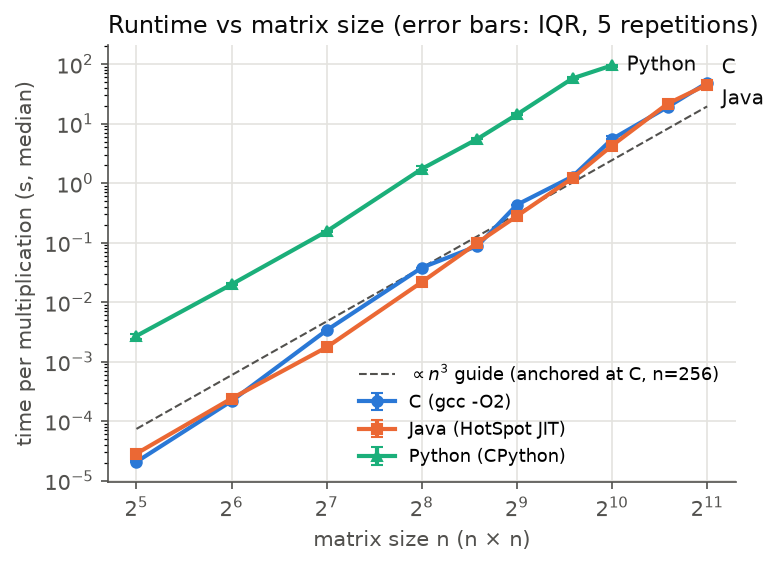
\includegraphics[width=0.74\linewidth]{../results/figures/fig_time_vs_n.png}
\caption{Median time per multiplication (log-log) with IQR error bars (5 repetitions; most bars are
smaller than the markers). The dashed line has slope 3. Python stops at $n=1024$ because $n=1536$
exceeded the 300\,s budget.}
\label{fig:time}
\end{figure}

\begin{table}[!htbp]
\centering\small
\caption{Runtime per multiplication: median over 5 measured repetitions, relative IQR
(IQR/median), median time divided by $n^3$ (ns per inner iteration), $2n^3$/median in GFLOP/s, and
batch size (multiplications per sample).}
\label{tab:time}
\TimeTable
\end{table}

\begin{figure}[!htbp]
\centering
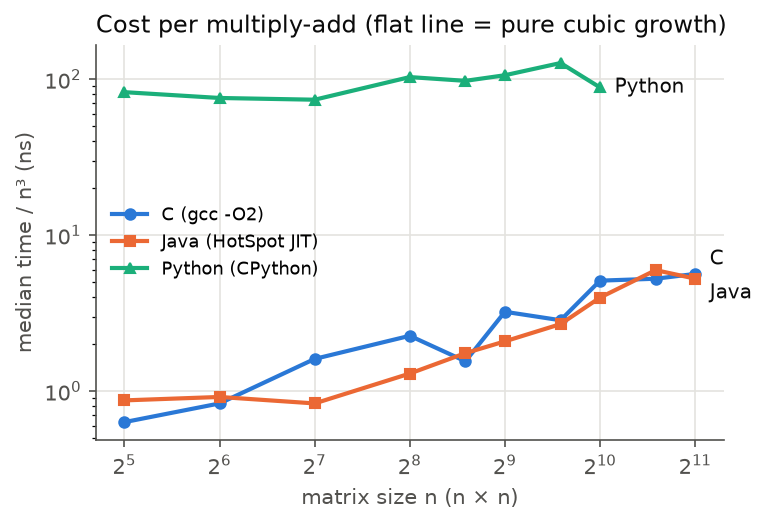
\includegraphics[width=0.72\linewidth]{../results/figures/fig_time_per_n3.png}
\caption{Median time divided by $n^3$. A horizontal line would mean exactly cubic growth.}
\label{fig:pern3}
\end{figure}

\begin{figure}[!htbp]
\centering
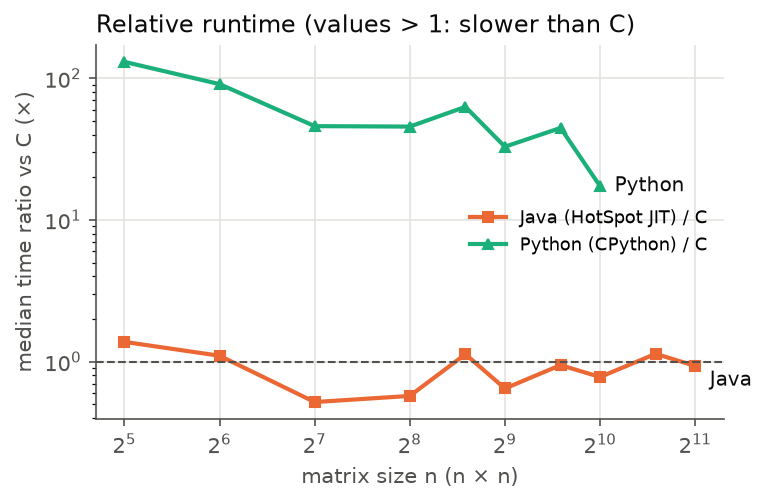
\includegraphics[width=0.70\linewidth]{../results/figures/fig_ratio_vs_c.png}
\caption{Median runtime relative to C at the same $n$.}
\label{fig:ratio}
\end{figure}

\FloatBarrier
\subsection{Memory}

\begin{figure}[!htbp]
\centering
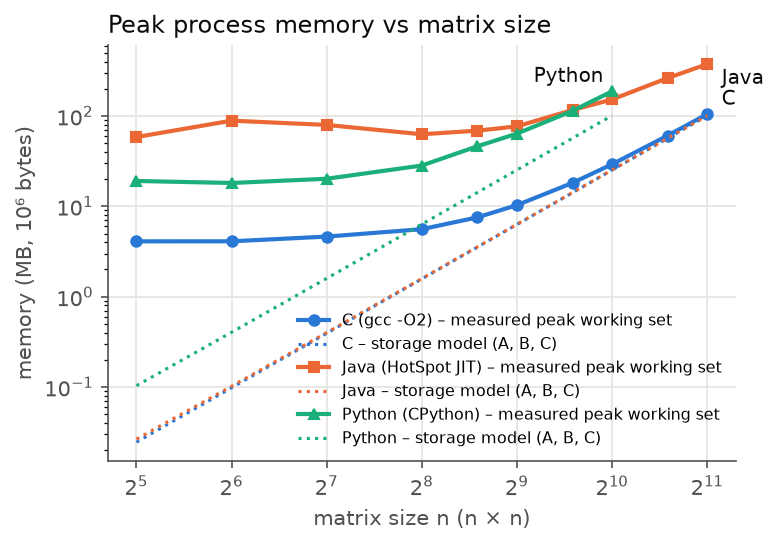
\includegraphics[width=0.74\linewidth]{../results/figures/fig_memory_vs_n.png}
\caption{Peak working set per process (solid) and analytical storage of $A$, $B$, $C$ (dotted; the C
and Java models almost coincide).}
\label{fig:mem}
\end{figure}

\begin{table}[!htbp]
\centering\small
\caption{Peak working set of the whole process (psutil) versus the storage model of the three
matrices. 1\,MB = $10^6$ bytes.}
\label{tab:mem}
\MemoryTable
\end{table}

For Java, the managed heap in use after the last repetition grew from 18--45\,MB at small $n$ to
176\,MB at $n=2048$, while the committed heap stayed at its initial 260\,MB (see
\texttt{results/raw/runs.csv}).

\FloatBarrier
\subsection{Limits}
\begin{itemize}[leftmargin=1.4em]
  \item \textbf{C and Java} completed every size up to the largest attempted, $n=2048$ (median 48.5\,s
        and 45.2\,s).
  \item \textbf{Python}'s largest completed size was $n=1024$ (median 95.1\,s); at $n=1536$ no
        multiplication finished within 300\,s and the run was stopped (peak working set 292\,MB at
        that point), so $n=2048$ was not attempted.
  \item \textbf{Memory:} no configuration came close to the 4\,GB memory budget.
\end{itemize}

\FloatBarrier
\subsection{Replication and supplementary experiments}

\concept{Replication}
After the main run, mid-size configurations were run again in a separate
session with the same protocol (Table~\ref{tab:rep}). Within the main session the relative IQR was
below 10\,\% for 21 of the 28 configurations (maximum 32\,\%, Java at $n=768$), but medians differed
between sessions by up to 58\,\%. The ordering of the languages was the same in both sessions at every
replicated size.

\begin{table}[!htbp]
\centering\small
\caption{Median time in the main run and in a later replication session
(\texttt{results/replication/}).}
\label{tab:rep}
\ReplicationTable
\end{table}

\concept{Row padding in C (layout hypothesis)}
To test whether cache conflicts caused by the
power-of-two row stride explain C's behaviour, \texttt{c/supplementary/matmul\_padded.c} runs the
\emph{same} kernel with each row stored $8n+16$ bytes apart (two unused doubles per row, mimicking
the Java header offset). The two layouts were measured alternately in one process to cancel drift.
The checksums of both layouts were identical at every size.

\begin{table}[!htbp]
\centering\small
\caption{Supplementary (not part of the controlled comparison): same C kernel, contiguous rows versus
rows padded by 16 bytes; 5 alternating repetitions, median.}
\label{tab:pad}
\PaddingTable
\end{table}

\begin{figure}[!htbp]
\centering
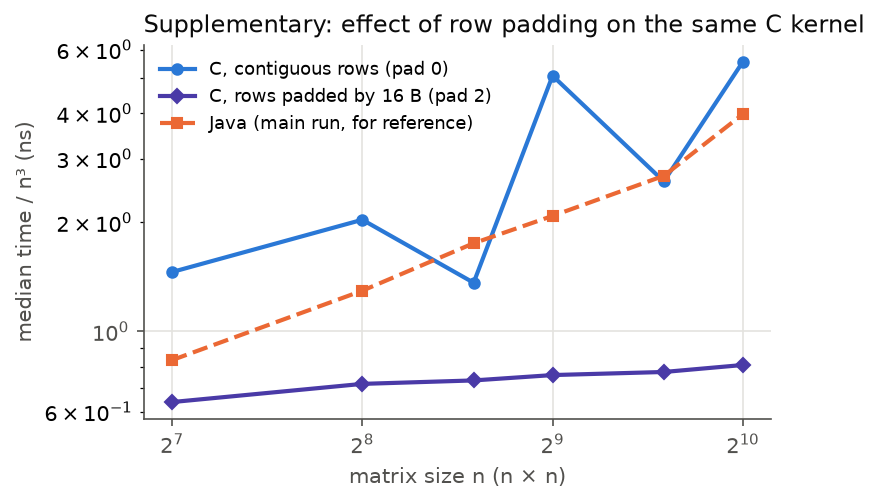
\includegraphics[width=0.70\linewidth]{../results/figures/fig_supp_padding.png}
\caption{Supplementary: time per inner iteration of the same C kernel with and without row padding.}
\label{fig:pad}
\end{figure}

\concept{GCC flags}
The same C source was also built with other flag sets (Table~\ref{tab:flags}).
Loop unrolling and \texttt{-O3} did not make the kernel faster than \texttt{-O2}.

\begin{table}[!htbp]
\centering\small
\caption{Supplementary: median time of the unmodified C kernel with different GCC flags (separate
session; variants run one after another, not interleaved).}
\label{tab:flags}
\FlagsTable
\end{table}

% =====================================================================
\FloatBarrier
\section{Discussion}

\concept{Growth and the cubic model (H1)}
The cubic model describes Python well: its cost per inner
iteration varied only between 74 and 127\,ns over a 32-fold range of $n$ (Fig.~\ref{fig:pern3}) and
the fitted exponent is 3.14. For C and Java, the exponent is clearly above 3 (3.50 and 3.73), so H1
is only partly supported. The algorithm still performs exactly $n^3$ iterations; what grows is the
\emph{cost per iteration}, from 0.6--0.95\,ns at $n\le64$ to 4--6\,ns at $n\ge1024$.

At $n=32$ all three matrices (24\,KB) fit in L1. The C value there, 0.63\,ns, matches roughly 3 cycles
per iteration at the CPU's 4.5\,GHz boost clock, which is consistent with the compiled loop
(\texttt{movsd}, \texttt{mulsd}, \texttt{addsd}; checked with \texttt{gcc -S}) being limited by the
latency of the floating-point additions chained through \texttt{s} \cite{fog,amd}. As $n$ grows, each
column walk of $B$ touches $n$ different cache lines, and the per-iteration cost rises when these no
longer fit in L1, L2 and then L3.

The fitted exponent therefore mixes the algorithmic $n^3$ with a size-dependent memory cost. It should
not be read as a property of the algorithm, and it depends on the size range.

\concept{Interpreter cost (H2)}
Python was 17--130$\times$ slower than C (Fig.~\ref{fig:ratio}),
which supports H2. Each Python inner iteration executes several bytecode instructions: two
subscriptions of nested lists, a multiplication and an addition that each allocate a new
\texttt{float} object, and loop control. This costs roughly 75--130\,ns, compared with a few
nanoseconds of memory stall in C.

Because the interpreter overhead dominates, Python is the least sensitive to cache effects and its
curve is the closest to a pure $n^3$ law. Its ratio to C \emph{falls} with $n$ only because C becomes
slower per iteration, not because Python becomes faster.

\concept{C versus Java: a layout effect, not a language ranking}
Contrary to H2, Java was faster than
C at most sizes from 128 to 1024. This held in both sessions, while C was faster at $n=384$ in both
(Tables~\ref{tab:time} and~\ref{tab:rep}). The C curve is irregular: per iteration, $n=384$ and
$n=768$ are cheaper than the power-of-two sizes next to them (Fig.~\ref{fig:pern3}).

This pattern points to conflict misses. In C, consecutive rows of $B$ are exactly $8n$ bytes apart, so
for $n=512$ the elements of a column are 4\,KB apart and map to a single L1 set (64 sets of 64-byte
lines). They also map to only 16 of the 1024 L2 sets, so only $16\times8=128$ of the 512 lines of
one column can stay in L2.

The supplementary padding experiment supports this explanation. Shifting every row by 16 bytes, with
no change to the arithmetic, made the same C code 1.9--6.9$\times$ faster, with the largest gains at
$n=512$ and $n=1024$ (Table~\ref{tab:pad}). Padded C was then faster than Java at every tested size and
had an almost flat cost of 0.64--0.81\,ns per iteration (Fig.~\ref{fig:pad}). Java's separately
allocated rows carry a 16-byte header, so its rows are normally not a power of two apart, which is a
plausible reason why Java avoids most of the penalty.

We did not inspect the JIT-generated code or the actual heap addresses, so this explanation of
Java's advantage is a supported hypothesis, not a proof. Unrolling (\texttt{-funroll-loops}) and
\texttt{-O3} did not speed up C (Table~\ref{tab:flags}), so instruction scheduling is unlikely to
explain the gap. That table also contains one unexplained observation: \texttt{-O0} was faster than
\texttt{-O2} at $n=512$ and $1024$. Explaining it would require hardware performance counters,
which were not used.

\concept{Memory (H3)}
Peak memory shows two regimes (Fig.~\ref{fig:mem}). For small $n$ it is the
runtime baseline: about 4\,MB for the C process, 18\,MB for CPython and 58--90\,MB for the JVM (heap,
JIT, class data). For large $n$ it follows $n^2$.

C's peak working set is the storage model plus about 4\,MB (104.7\,MB measured versus 100.7\,MB
modelled at $n=2048$). Python's storage model is four times C's (32 instead of 8 bytes per element),
which supports H3. Its measured peak (187\,MB at $n=1024$) exceeds the model because the interpreter
baseline is added and because the previous result matrix remains referenced while the next one is
computed in the repetition loop.

The JVM's peak (374\,MB at $n=2048$) is well above both its storage model (101\,MB) and the heap in use
(176\,MB). G1 lets garbage from earlier repetitions accumulate before collecting it, and the JVM does
not return committed memory to the OS immediately. The JVM's footprint is therefore governed by GC
policy and heap settings (\texttt{-Xmx4g}) rather than by the matrices alone. Memory never limited
any run; time was the binding constraint for Python.

\concept{Limitations}
\begin{enumerate}[label=(\roman*), leftmargin=2.2em]
  \item One laptop with a ``Balanced'' power plan and dynamic frequency scaling. Medians varied by up
        to 58\,\% between sessions (Table~\ref{tab:rep}), much more than the within-session IQR.
        Comparisons are reliable for ratios of several times (Python versus C/Java, padded versus
        unpadded C), but small differences between C and Java, such as at $n=384$, are within this
        drift. Interleaving languages within a session, fixing the CPU frequency and running more
        sessions would reduce it.
  \item Five repetitions per configuration, in one process each. Between-process (JIT) variance for
        Java was only sampled through the replication.
  \item The peak working set is sampled every 20\,ms. It is an OS high-water mark, so short peaks are
        not lost, but it includes runtime overheads and is not comparable to the Java heap metric.
  \item The explanations of cache behaviour rely on layout arithmetic and the padding experiment, not
        on hardware counter measurements.
  \item Results hold for the i-j-k order and binary64. Other loop orders, which Assignment~2 will
        study, change the access pattern of $B$ completely.
\end{enumerate}

% =====================================================================
\Needspace{22\baselineskip}
\section{Conclusions}
\begin{titledbox}{Key findings}
On this machine and with these settings:
\begin{itemize}[leftmargin=1.2em]
  \item The same $O(n^3)$ triple loop gave \textbf{bitwise-identical results} in C, Java and Python.
  \item CPython was \textbf{one to two orders of magnitude slower} than C and Java (17--130$\times$
        relative to C) and could not complete $n=1536$ within 300\,s.
  \item C and Java differed by \textbf{less than a factor of two}, in both directions.
  \item Python's runtime followed the \textbf{cubic model} closely because interpretation dominates
        each iteration. C's and Java's runtime grew \textbf{faster than $n^3$} over the tested range
        because the memory cost per iteration increases as the matrices leave the caches.
  \item The comparison between C and Java depended more on \textbf{memory layout} than on the
        language: a 16-byte row padding made the same C code up to 6.9$\times$ faster.
  \item Memory grew as \textbf{$n^2$} once runtime baselines were exceeded, with Python using about
        four times C's storage per element and the JVM adding a large, GC-dependent overhead.
\end{itemize}
\end{titledbox}

\concept{Open questions}
A hardware-counter confirmation of the conflict-miss explanation, the reason for the
fast \texttt{-O0} build, and how much of the session-to-session variation comes from frequency
scaling. The validated implementations, inputs and scripts are reused as the baseline in
Assignment~2.

% =====================================================================
\section*{Reproducibility materials}
Repository: \url{\RepoURL}. It contains:
\begin{itemize}[leftmargin=1.4em]
  \item source code: \texttt{c/}, \texttt{java/}, \texttt{python/};
  \item configuration: \texttt{config/benchmark\_config.json};
  \item input generation (\texttt{scripts/generate\_inputs.py}) and the build, benchmark, validation
        and analysis scripts;
  \item all raw measurements: \texttt{results/raw/}, \texttt{results/replication/},
        \texttt{results/supplementary/};
  \item a README with exact build and run commands and dependency versions.
\end{itemize}

\section*{Use of generative AI}
Claude (Anthropic) was used to help write the implementations, the benchmarking and analysis scripts,
and a draft of this report. All numbers in this report come from running the code on the machine
described above; the raw data are included.

% =====================================================================
\begin{thebibliography}{99}\small\sloppy
\setlength{\itemsep}{3pt}
\bibitem{golub} G.~H. Golub and C.~F. Van~Loan, \emph{Matrix Computations}, 4th ed. Baltimore, MD, USA: Johns Hopkins Univ. Press, 2013.
\bibitem{higham} N.~J. Higham, \emph{Accuracy and Stability of Numerical Algorithms}, 2nd ed. Philadelphia, PA, USA: SIAM, 2002.
\bibitem{ieee754} \emph{IEEE Standard for Floating-Point Arithmetic}, IEEE Std 754-2019, 2019.
\bibitem{jep306} J.~Darcy, ``JEP 306: Restore Always-Strict Floating-Point Semantics,'' OpenJDK, 2021. [Online]. Available: \url{https://openjdk.org/jeps/306}
\bibitem{lam} M.~S. Lam, E.~E. Rothberg, and M.~E. Wolf, ``The cache performance and optimizations of blocked algorithms,'' in \emph{Proc. ASPLOS-IV}, 1991, pp.~63--74.
\bibitem{drepper} U.~Drepper, ``What every programmer should know about memory,'' Red Hat, Inc., 2007. [Online]. Available: \url{https://people.freebsd.org/~lstewart/articles/cpumemory.pdf}
\bibitem{hennessy} J.~L. Hennessy and D.~A. Patterson, \emph{Computer Architecture: A Quantitative Approach}, 6th ed. Cambridge, MA, USA: Morgan Kaufmann, 2017.
\bibitem{amd} Advanced Micro Devices, ``Software Optimization Guide for AMD Family 19h Processors,'' Pub. no. 56665, 2020.
\bibitem{fog} A.~Fog, ``Instruction tables: Lists of instruction latencies, throughputs and micro-operation breakdowns for Intel, AMD and VIA CPUs,'' Technical University of Denmark. [Online]. Available: \url{https://www.agner.org/optimize/}
\bibitem{georges} A.~Georges, D.~Buytaert, and L.~Eeckhout, ``Statistically rigorous Java performance evaluation,'' in \emph{Proc. OOPSLA}, 2007, pp.~57--76.
\bibitem{psutil} G.~Rodola, ``psutil documentation,'' 2026. [Online]. Available: \url{https://psutil.readthedocs.io/}
\end{thebibliography}

\end{document}
